% Chapter 5
\chapter{Deep Graph Kernels} % Main chapter title

\label{Chapter5} % For referencing the chapter elsewhere, use \ref{Chapter1} 

\lhead{Chapter5. \emph{Deep Graph Kernels}} % This is for the header on each page - perhaps a shortened title

%----------------------------------------------------------------------------------------
Over recent years, graph kernels are one the promising candidate for problem related to graph isomorphism. Graph Kernels are based on the comparison of graph-substructures via kernels. The graph-substructure including walks, path, subtrees, graphlets and cyclic patterns have been widely used to construct kernels. However, kernels on these substructures are either computationally expensive, NP-hard to determine, limited in their expressiveness or applicable to  just a small
subset of graphs rather all graphs. Existing graph kernels have difficulties with reaching at least one of these goals.

An emerging line of research, consisting in designing meaningful kernels on structured data, produced promising results in cheminformatics, bioinformatics, computer vision and natural language processing. The graph kernels together with techniques from natural language processing and computer vision  have recently received an increased attention, and showed good performances for classification of small molecules \citep{Mahe2004}. In very recent years, lots of research has been developed around deep learning architectures that allow for higher level abstractions for representing and understanding graph data \citep{Perozzi2014}.

Deep learning is method based on learning representations of data, which attempt to model high-level abstractions in data by using multiple processing layers, with complex structures or otherwise, composed of multiple non-linear transformations. By using deep learning, Perozzi et al.\citep{Perozzi2014} proposed DeepWalk, which uses local information obtained from truncated random walks to learn social representations of vertices of graphs. Motivating from DeepWalk, Yanardag and Vishwanathan \citep{Yanardag2015} work focuses on learning similarities
between structured objects, such as graphs and strings, instead of nodes of the single graph. However, the adoption of deep learning in graphs isomorphisms has not been adequately investigated yet. 

\section{Background}

Deep Graph Kernels \citep{Yanardag2015} is not so deep learning frame work to learn latent representations of sub-structures for graphs, which are not independent. The framework leverage on the dependency information between sub-structures by learning their latent representations. To motivate our discussion of using deep graph kernels, we first try to explain the problem associated with general graph kernels representation.

\section{Representation Problem}

Graph Kernels are produced using R-convolution, where a graph is to recursively decomposed into into “atomic” sub-structures to define a kernels between them.  Mathematically, It can be expressed as:

%
\begin{equation}
K(G_{1}, G_{2}) = {\Bigg \langle \Phi(G_{1}), \Phi(G_{1}) \Bigg \rangle}_{\mathcal{H}}
\label{eq:dgk}
\end{equation}
%

Where, $\Phi(G)$ is denote a vector which contains counts of atomic sub-structures. 

The representation in the equation \ref{eq:dgk} suffers from two basic problems. First, the sub-structure are not independent. Second, the dimension of the feature space often grows exponentially, as substructure grows, which leads to "diagonal dominance" \citep{Kandola2003}, that is, a given graph is similar to itself but not to any other graph in the dataset. But, we need a kernel matrix where all entries belonging to a class are similar to each other, and dissimilar to everything else. 

\section{Deep Framework}

To alleviate the representation problem, we define alternative graph kernel as:

%
\begin{equation}\label{eq:pdgk}
K(G_{1}, G_{2}) = \Phi(G_{1})^{T} \mathcal{M} \Phi(G_{1})
\end{equation}
%
 
where $\mathcal{M}$ represents a $|\mathcal{N}|\times |\mathcal{N}|$ positive semi-definite matrix that encodes the relationship between sub-structures and $\mathcal{N}$ represents the vocabulary of sub-structures obtained from the training data. Now, the important task is design $\mathcal{M}$, which can be computed by learning latent representations of sub-structures or by edit-distance relationship between sub-structures.

\section{Methodology} 

The $\mathcal{M}$ is computed by learning  the latent representations of
sub-structures by techniques such as Neural language models,  Continuous bag-of-words (CBOW) and Skip-gram model (SG) \citep{Yanardag2015}.

\subsection{Skip-Gram}
First, we review the representative Skip-Gram \citep{Milkov2013} \footnote{The google tool, \textit{Word2Vec} provides a fast, multi-threaded implementation of both SG and CBOW:https://code.google.com/p/word2vec/}. architecture in language modelling before transforming the ideas to learn representations of sub-structures. 

The SG model maximizes co-occurrence probability among the words that appear within a given window.  More precisely, SG model tries to minimize the following objective function: 
%
\begin{equation}
\mathcal{L}_{SG} = \sum_{t=1}^{T} \log P(w_{t-c}, \cdots , w_{t+c}|w_{t})
\label{eq:SG}
\end{equation}
%
where, $P(w_{t-c}, \cdots , w_{t+c}|w_{t})$ is computed as $\prod_{-c\leq j\leq c, j \neq 0} P(w_{t+j}|w_{t})$. Furthermore, 

%
\begin{equation}
P(w_{t+j}|w_{t}) = \frac{\exp(v^{\intercal}_{{w}_{t}} v^{\prime}_{{w}_{t}})}{\sum_{w=1}^{\mathcal{V}}\exp (v^{\intercal}_{{w}_{t}} v^{\prime}_{{w}_{t}})}
\end{equation}
%

Hierarchical softmax or negative sampling are two efficient algorithms that are used in training SG and CBOW  \citep{Yanardag2015}.

\section{Deep Graph Kernels}

The language modeling and deep learning techniques was used to compute $\mathcal{M}$ with intuition that different sub-structures compose graphs in a similar way that different words form sentences when used together. The list of decomposed sub-structures for each graph is then treated as a sentence that is generated from a vocabulary $\mathcal{V}$  where vocabulary $\mathcal{V}$ simply corresponds to the unique set of observed sub-structures in the training data. 

The linear co-occurrence relationship of sub-structure is created using modified random sampling scheme, taking account of neighborhoods. That is, whenever we randomly sample a graphlet $G$, we also sample its immediate neighbors. Then is corpus is generated according to particular graph kernels, for example, for shortest graph kernels, whenever shortestpath sub-structure is generated, all possible shortest-path sub-structures are also collected that share the same source node, and treat them as co-occurred.

\subsection{Corpus Generation}

Most of the graph kernels \citep{Vishwanathan2010} are designed for unlabeled graphs or graphs with a complete set of discrete node labels
, but graphs with continuous node attributes is catching up fast \citep{Feragen2013}. But these graph kernels can only handle graphs with complete label or attribute information in a principled manner. These may be efficient, but for specific graph and if flexible, computation is memory and/or time consuming. The propagation kernels by  \citep{Neumann2015} overcomes all the above problems. We exploit the propagation kernels in the deep framework to have similarity index between two graph. The propagation kernels measure the similarity between two graphs by comparing node label or attribute distributions after each step of an appropriate random walk.

The corpus is generated for propagation kernels \citep{Neumann2015}, which is explained in section \ref{sec:PGK}. Since, the propagation kernels are based on monitoring how information spreads through a set of given graphs. We use early-stage distributions from propagation
schemes such as random walks to capture structural information encoded in node labels, attributes, and edge information. In simple words, propagation kernels intuitively count common sub-distributions induced
after each iteration of running inference in two graphs. We collect all possible sub-distributions that share the same source node, and treat them as co-occurred. Therefore, sub-distributions which have similar labels will acquire similar representations. We differ from earlier studies in using propagation kernels, which is efficient than random walk, shortest path, graphlet and Weisfeiler-Lehman subtree kernel.

\subsection{Model Building and Training}
\label{ssec:MBT}
Once corpus is generated, the model is build by using  Skip-gram algorithms and trained with negative sampling as explained in the base reference \citep{Yanardag2015}. 

If $s$ represent an arbitrary sub-structure from a vocabulary $\mathcal{V}$, and $\phi_{s}$ represent learned vector representation of $s$. Matrix $\mathcal{M}$ is calculated such that, each entry on the diagonal is $\mathcal{M}_{ii}$ computed as $\big \langle \phi_{i},\phi_{i} \big \rangle$ where $\phi_{i}$ corresponds
to learned d-dimensional hidden of sub-sequence $i$ and $\mathcal{M}_{ii}$
where $i = $j and $1 \leq i \leq |\mathcal{V}|$ (resp. $j$). After computing the $\mathcal{M}$ matrix, it is plugged in Equation \ref{eq:pdgk} to get deep graph kernels. The similarity index $SI_{DGP}(G_{1}, G_{2})$ is calculated by normalising the \ref{eq:pdgk}.


\subsection{Experiments}
We compare our framework with the representative instances of
major families of graph kernels as discussed in \citep{Yanardag2015}. The similarity index is calculated as discussed in section \ref{ssec:MBT}. The Matlab code of the propagation kernels was obtained from \citep{Neumann2015}, which was then coded in python. The correlation between transaction network structure and market price is depicted by figure \ref{fig:ds}. It shows better correlation with the network, as compared to similarity index calculated by other graph kernels without using deep framework. 

\begin{figure}[ht]
\begin{center}
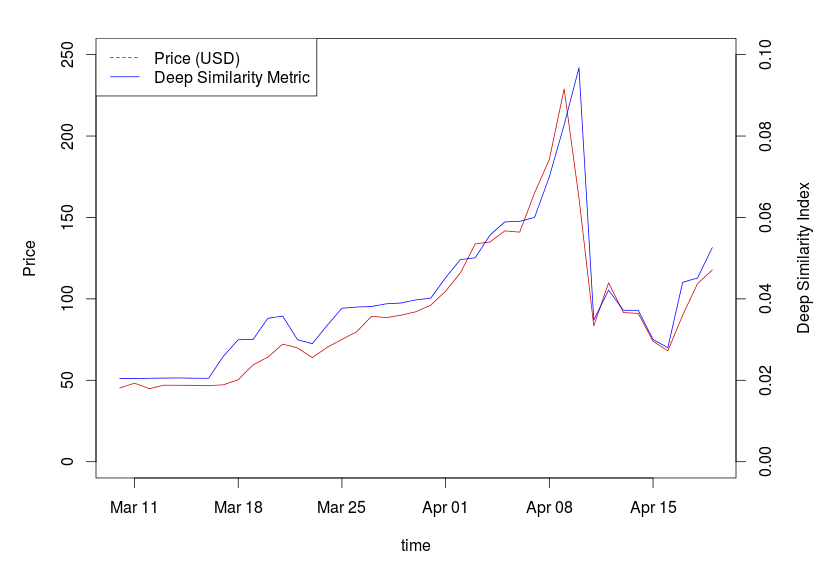
\includegraphics[width=0.8\textwidth]{./Figures/ds.png}
\caption{Deep Similarity}
\label{fig:ds}
\end{center}
\end{figure}

\section{Result and Discussions}
As per Bitcoin’s ”Metcalfe’s Law”, there is strong correlation between
market cap (transactions/day) and the square of the number of
transactions. As our graph is weighted network, where weight
represents the transactions between two agents, our results too
supports Metcalfe’s Law. We are able to show how structural changes in the network accompany significant changes (Quantitative Measure) in the
exchange price of bitcoins.

\section{Conclusions}
 In this study, we extend the quite novel framework for graph kernels inspired by latest advancements in natural language processing and deep learning. We extend the seminal work \citep{Yanardag2015} by introducing propagation kernels, which takes account of attributed graphs with continuous values. As expected, our deep graph kernels outperforms its best base variants in terms of capturing correlation between newtork structure and market price.
 
\section{Summary}
This chapter propose a general framework that learns hidden representations of sub-structures used in graph kernels, inspired
by deep graph kernels \citep{Yanardag2015}. Then, the framework  is demonstrated on propagation kernels, which performs better than normal kernels. The above framework is applied to derive deep variants of
string kernels. Then new graph kernel is used to calculate similarity index, which is plotted to find correlation between network structure and market price.

%----------------------------------------------------------------------------------------


